\subsection{Niveau 2 - Balayer}

\begin{center}
\begin{figure}[!h]
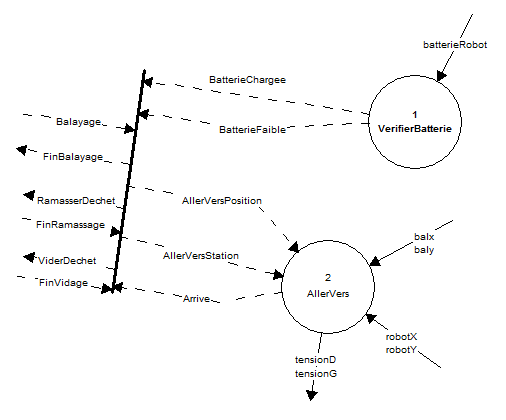
\includegraphics[height=10cm]{\PIXPATH/balayer}
\caption{Niveau 2 - Détecter}
\end{figure}
\end{center}


\subsubsection{Diagramme états-transitions}

\begin{center}
\begin{figure}[!h]
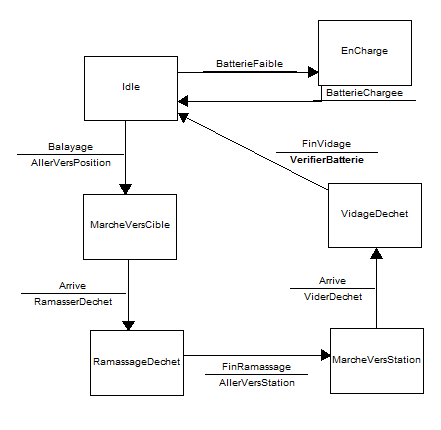
\includegraphics[height=8.5cm]{\PIXPATH/balayer_etat}
\caption{Diagramme états-transitions}
\end{figure}
\end{center}

\subsubsection{Processus primitifs - C-Spec}

\begin{description}
	
	\item \textbf{VerifierBatterie}
		\begin{tabbing} 
		\textbf{IN} : batterieRobot \\
		\textbf{OUT} : BatterieChargee, BatterieFaible \\
		si \=($batterieRobot \leq 0.15$) \\
			\>BatterieFaible emis \\
		sinon si ($batterieRobot \geq 0.95$ \\
			\>BatterieCahrgee emis \\
		fin si 
		\end{tabbing}


\end{description}

\vfill
\pagebreak

